\documentclass[compress,red]{beamer}
\usepackage{etex}
\mode<presentation>
%\usetheme{Warsaw}
%\usepackage[applemac]{inputenc}  %les accents pour mac. for xelatex, pdflatex is used here
\usepackage{caption}
\captionsetup{font=small}
\captionsetup{labelformat=empty}
\usepackage[list=true]{subcaption}
%\usepackage[demo]{graphicx}  % beamer already load this
\usepackage{multicol}
  \usepackage{animate}
%  \usepackage{movie 15}
 \usepackage{amsmath}
 \usepackage{epsfig}
\usepackage[all,knot]{xy}
\xyoption{arc}
\usepackage{url}
\usepackage{array,ragged2e}
\usepackage{multimedia}
\usepackage{hyperref}
\usepackage{setspace}
\usepackage{multirow} 

\begin{document}


\begin{frame}
 \frametitle{Approach}
{\small
Given a phylogenetic tree, we define the following Random Variables, \\
\vspace{0.3cm}
$T_i:$ branching time $i$ of the phylogenetic tree\\
$X_i:$ binarary variable equal to $1$ if the process $i$ is an speciation, and $0$ if is an extinction. \\
\vspace{0.2cm}
Then, we define the phylogenetic tree as a data frame $Y = \{X_i,T_i\}$.
\vspace{0.1cm}
}

We suppose that the random variable $T$ follows an exponential distribution with parameter $\nu = \sum \lambda_i + \mu_i$ where $\lambda_i$ and $\mu_i$ are the speciation and extinction rates, and $X_i$ follows a Bernoulli distribution with parameter $p_i = \lambda_i / \nu$ corresponding to the probability of speciation (or extinction) of specie $i$. \\
\vspace{0.2cm}
Thus, we write the likelihood of the phylogenetic tree as 

$$L(Y;\lambda,\mu) = \prod_{i=1}^N \nu e^{-\nu t_i} p_i $$

where $N$ es the number of branching times on the phylogenetc tree. \\
%\vspace{0.11cm}
%Moreover, we assumme the rates $\lambda = f(cov)$, $\mu = f(cov)$.
\end{frame}


\begin{frame}[shrink]
 \frametitle{Some simulations}
 
 Moreover, we assumme the rates $\lambda = f(cov)$, $\mu = f(cov)$. In the simulation bellow we have a simple model $ \lambda = exp\{\theta_0 + \theta_1 b\} $, $\mu = exp\{\varphi_0 + \varphi_1 b\} $ 

\begin{table}[ht]
\centering
\begin{tabular}{r|rrrrr}
  \hline
  n = 896 & real value & mean & median & min & max \\ 
  \hline
$\theta_1$  & 3.00 & 3.05 & {\color{blue}3.03} & 0.39 & 6.00 \\ 
  $\theta_2$  & 4.00 & 0.61 & {\color{blue}3.85} & -4136.88 & 949.77 \\ 
  $\phi_1$  & 1.00 & 0.68 & {\color{blue}0.81} & -26.92 & 24.46 \\ 
  $\phi_2$  & 2.00 & 5.00 & {\color{blue}1.80} & -2712.26 & 2164.94 \\ \hline
%   $\theta_1$ & 9137 & 3.00 & 3.05 & {\color{blue}3.03} & 0.12 & 6.58 \\ 
%   $\theta_2$ & 9137 & 4.00 & 0.59 & {\color{blue}3.79} & -6129.01 & 3038.34 \\ 
%   $\phi_1$ & 9137 & 1.00 & 1.99 & {\color{blue}0.87} & -33.06 & 8901.94 \\ 
%   $\phi_2$ & 9137 & 2.00 & 0.09 & {\color{blue}1.59} & -18755.83 & 10629.12 \\ 
%    \hline
\end{tabular}
\end{table}

\begin{figure}
\centering
 \subcaptionbox{$\theta_0$}{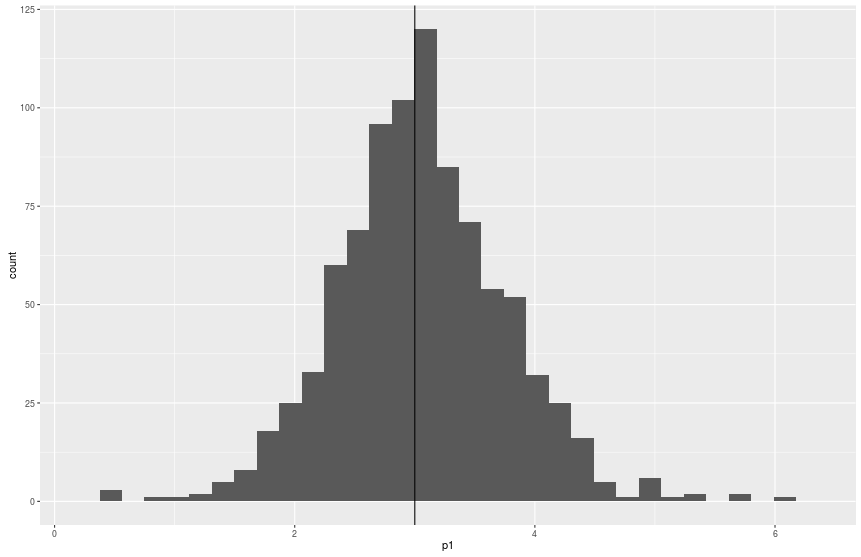
\includegraphics[width=0.3\textwidth]{h1}}
 \subcaptionbox{$\theta_1$}{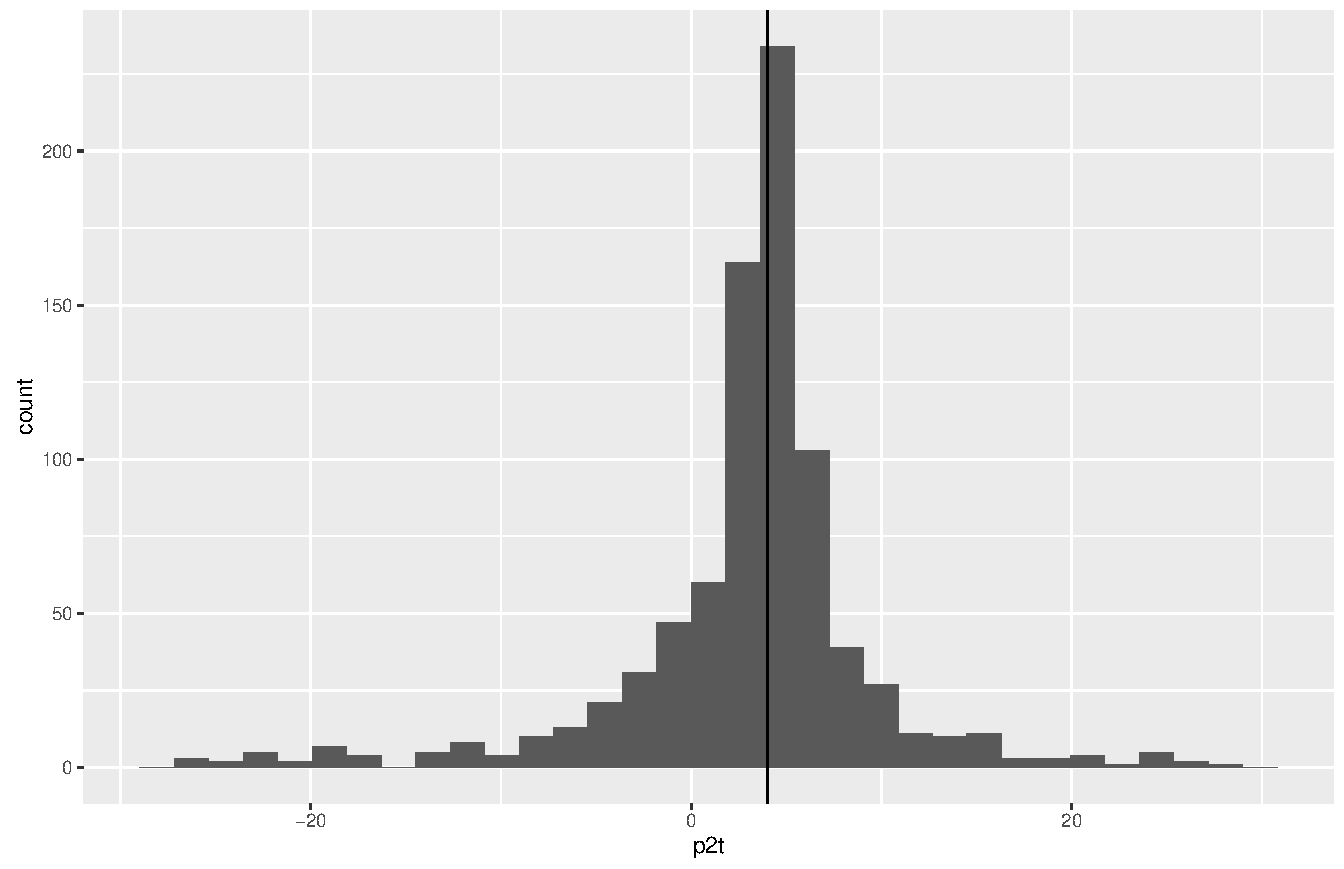
\includegraphics[width=0.3\textwidth]{h2}}\\
  \subcaptionbox{$\varphi_0$}{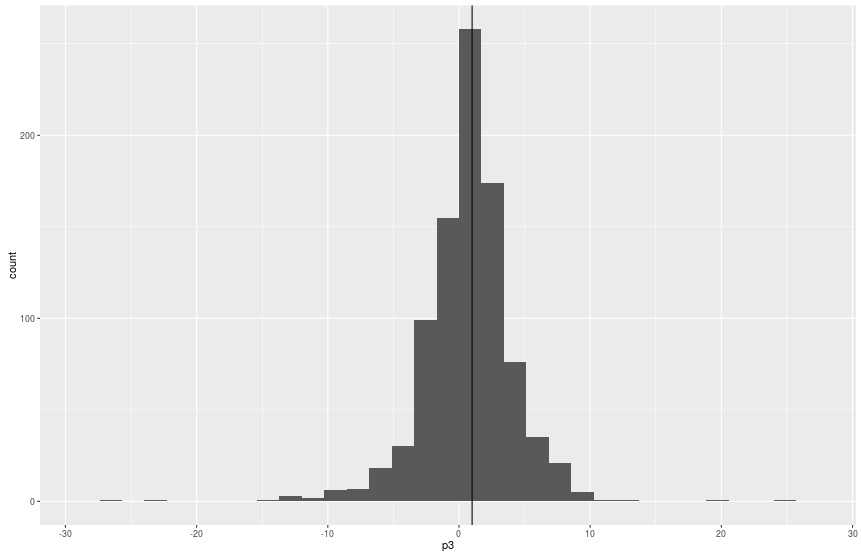
\includegraphics[width=0.3\textwidth]{h3}}
 \subcaptionbox{$\varphi_1$}{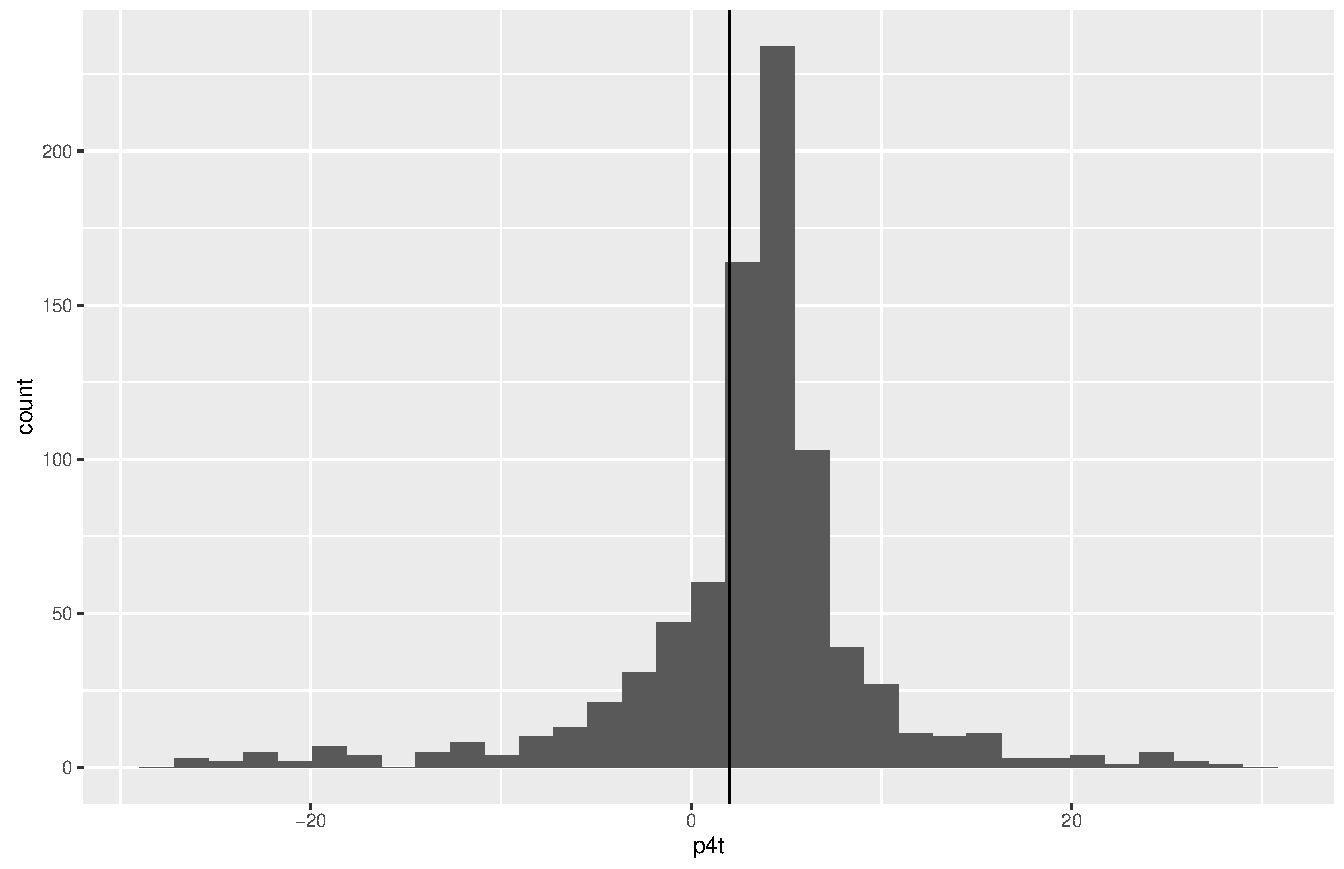
\includegraphics[width=0.3\textwidth]{h4}}
% \caption{Histograms of the estimated values. The black vertical line corresponds to the real values.} 
\end{figure}

%$ \eta = \langle x , \theta \rangle $

\end{frame}

\begin{frame}

\frametitle{GLM \& IWLS}
{\small
Linear models of the form 

	$$ E(Y_i) = \mu_i = \bold{x}_i^T \beta_i; \qquad Y_i \sim N(\mu_i,\sigma^2), $$

are widely used for their well known estimation methods and computational convinience.\\
\vspace{0.1cm}
Advances in statistical theory and computers software allow us to use methods analogous to those developed for linear models in the following more general situation: 

\begin{enumerate}
\item Response variables have distributions other than the Normal distribution (they may even be categorical rather than continuous). 
\item Rlationship between the response and the explanatory variable need not be the simple linear form above. 
\end{enumerate}
}

Usually, for GLM,  maximun likelihood estimators are obtained by an {\bf iterative weighted least squares} procedure, 

$$ X^TWXb^{(m)} = X^T W z. $$ 

\end{frame}



\end{document}

